\documentclass[11pt]{article}
\usepackage[margin=1in]{geometry}
\usepackage{graphicx}
\usepackage{amsmath}
\usepackage{booktabs}
\usepackage{hyperref}
\usepackage{listings}
\usepackage{xcolor}

\lstset{
    basicstyle=\ttfamily\small,
    breaklines=true,
    frame=single,
    language=Python
}

\title{Machine Learning Assignment: Transformer Analysis}
\author{Student ID: 24377372}
\date{\today}

\begin{document}

\maketitle

\section*{Introduction}

This assignment explores the GPT transformer architecture through systematic experimentation on model downsizing, architectural component analysis, and generalization testing. I trained multiple model configurations on a child speech dataset and evaluated their performance on in-distribution and out-of-distribution test sets.

\section*{(i.a) Dataset Analysis}

I analyzed three datasets provided: child speech training set, child speech test set, and Shakespeare text.

\subsection*{Child Speech Training Set}

\textbf{Characteristics:} The training dataset contains 246,982 characters across 10,001 lines with 55,076 words. The vocabulary consists of only 40 unique characters, representing a simple language structure typical of early childhood speech patterns.

\textbf{Content Analysis:} The dataset comprises short, repetitive phrases such as ``I see bird,'' ``No mine,'' ``More bubbles,'' indicating vocabulary and grammatical structures of 2-3 year old children. The text exhibits high redundancy with only 88 unique words, suggesting strong statistical patterns suitable for language modeling.

\textbf{Vocabulary:} The character set includes lowercase and uppercase letters (a-z, A-Z), space, and newline: \texttt{'\textbackslash nABCDGHILMNRSUWYabcdefghijklmnoprstuvwy'}. Notably absent are numbers and most punctuation, reflecting the simple conversational nature.

\subsection*{Child Speech Test Set}

\textbf{Size:} 24,113 characters across 1,001 lines with 5,347 words. The test set maintains identical vocabulary (40 characters, 88 unique words) and similar statistical properties to the training set (average line length 24.09 vs 24.70 characters), confirming it is in-distribution.

\subsection*{Shakespeare Dataset}

\textbf{Size:} 1,115,394 characters (4.5× larger than training), 40,001 lines, 202,651 words with 25,670 unique words.

\textbf{Vocabulary:} 65 unique characters including punctuation (\texttt{!?\$\&',-.3:;}), numbers, and full alphabet. The 25 additional characters not present in training vocabulary create a distribution shift.

\textbf{Linguistic Complexity:} Elizabethan English with complex syntax, archaic vocabulary (``thy,'' ``forsooth''), and formal dialogue structure contrasts sharply with simple child speech, making this an out-of-distribution test set.

\section*{(i.b) Model Downsizing to <1M Parameters}

\textbf{Original Model:} The baseline \texttt{gpt.py} contains 10.77M parameters with configuration: \texttt{n\_embd}=384, \texttt{n\_head}=6, \texttt{n\_layer}=6, \texttt{block\_size}=256.

\textbf{Rationale for Downsizing Strategy:} I chose to primarily reduce the embedding dimension because it affects parameter count multiplicatively across all model components. The embedding dimension influences:
\begin{itemize}
    \item Token and position embedding tables: $\text{vocab\_size} \times \text{n\_embd} + \text{block\_size} \times \text{n\_embd}$
    \item Attention projections: Each of 3 projections (key, query, value) per head scales with n\_embd
    \item Feed-forward layers: Hidden dimension is $4 \times \text{n\_embd}$
    \item Output projection: $\text{n\_embd} \times \text{vocab\_size}$
\end{itemize}

\textbf{Selected Configuration:} 
\begin{itemize}
    \item \texttt{n\_embd} = 96 (reduced from 384)
    \item \texttt{n\_head} = 4 (reduced from 6)
    \item \texttt{n\_layer} = 4 (reduced from 6)
    \item \texttt{block\_size} = 256 (unchanged)
    \item \textbf{Total Parameters:} 0.478M
\end{itemize}

This configuration maintains reasonable depth (4 layers) and multi-head attention (4 heads) while drastically reducing capacity through the embedding dimension. For simple child speech with limited vocabulary (40 characters), a 96-dimensional representation should provide sufficient expressiveness.

\section*{(i.c) Three Downsizing Configurations}

I explored three distinct downsizing strategies, each targeting different architectural components. The rubric requires at least two different ways of downsizing; I present three to provide comprehensive analysis:

\subsection*{Configuration 1: Reduced Embedding (0.478M parameters)}

\textbf{Strategy:} Aggressively reduce embedding dimension while maintaining depth.

\textbf{Hyperparameters:} \texttt{n\_embd}=96, \texttt{n\_head}=4, \texttt{n\_layer}=4, \texttt{block\_size}=256

\textbf{Training Results:}
\begin{itemize}
    \item Initial loss: 3.69 (baseline random uniform over 40 characters)
    \item Final training loss: 0.3435
    \item Final validation loss: 0.3464
\end{itemize}

\textbf{Generated Text Quality:} The model generates coherent child speech patterns:
\begin{verbatim}
No mine More bubbles
Mama Ma Read book
More buoore before bed More more
I jump high More more
No like it What is that
I want that Read book
All gone No nap
\end{verbatim}
The output captures common phrases (``More bubbles,'' ``Read book,'' ``No nap'') and maintains grammatical simplicity. Some repetition occurs (``More more'') and occasional misspellings (``buoore'' instead of ``before''), but overall the model learned the statistical patterns of child speech vocabulary and sentence structure.

\subsection*{Configuration 2: Shallow Network (0.439M parameters)}

\textbf{Strategy:} Minimize network depth to reduce parameters.

\textbf{Hyperparameters:} \texttt{n\_embd}=128, \texttt{n\_head}=4, \texttt{n\_layer}=2, \texttt{block\_size}=256

\textbf{Rationale:} With only 2 layers, the network has limited depth for learning complex patterns, but wider embeddings (128 vs 96) provide more representational capacity per layer. This tests whether depth or width matters more for this task.

\textbf{Training Results:}
\begin{itemize}
    \item Final training loss: 0.3413
    \item Final validation loss: 0.3447
\end{itemize}

\textbf{Generated Text Quality:} Configuration 2 produces similar quality output:
\begin{verbatim}
I draw Come here
More bubbbles Night night
I run fast No stop
Bath time I jump high
I did it No touch
\end{verbatim}
The shallow 2-layer architecture still captures child speech patterns effectively. The output shows good phrase diversity and maintains coherence, suggesting that for this simple dataset, width (128-dim embeddings) compensates for reduced depth.

\subsection*{Configuration 3: Balanced Reduction (0.612M parameters)}

\textbf{Strategy:} Reduce both context window and layer count proportionally.

\textbf{Hyperparameters:} \texttt{n\_embd}=128, \texttt{n\_head}=4, \texttt{n\_layer}=3, \texttt{block\_size}=64

\textbf{Rationale:} Child speech phrases are typically short (average 24 characters per line). A context window of 64 characters should capture 2-3 phrases, sufficient for pattern learning while saving parameters in the position embedding table.

\textbf{Training Results:}
\begin{itemize}
    \item Final training loss: 0.3811
    \item Final validation loss: 0.3832
\end{itemize}

\textbf{Generated Text Quality:} Configuration 3 with reduced context window produces:
\begin{verbatim}
No mine Daddy read me dinosaur book before bed
Mama I want play with big Read book
Look moon Go park
Night night Go park
Big hug No mine
\end{verbatim}
The output maintains coherence and generates longer phrases (``Daddy read me dinosaur book before bed''). The 64-character context window appears sufficient for capturing child speech patterns, though the loss is slightly higher than Configs 1 and 2.

\subsection*{Comparative Analysis}

\textbf{Loss Curves:} Figure~\ref{fig:training-comparison} visualizes the loss trajectories for all three downsized configurations.

\begin{figure}[h]
\centering
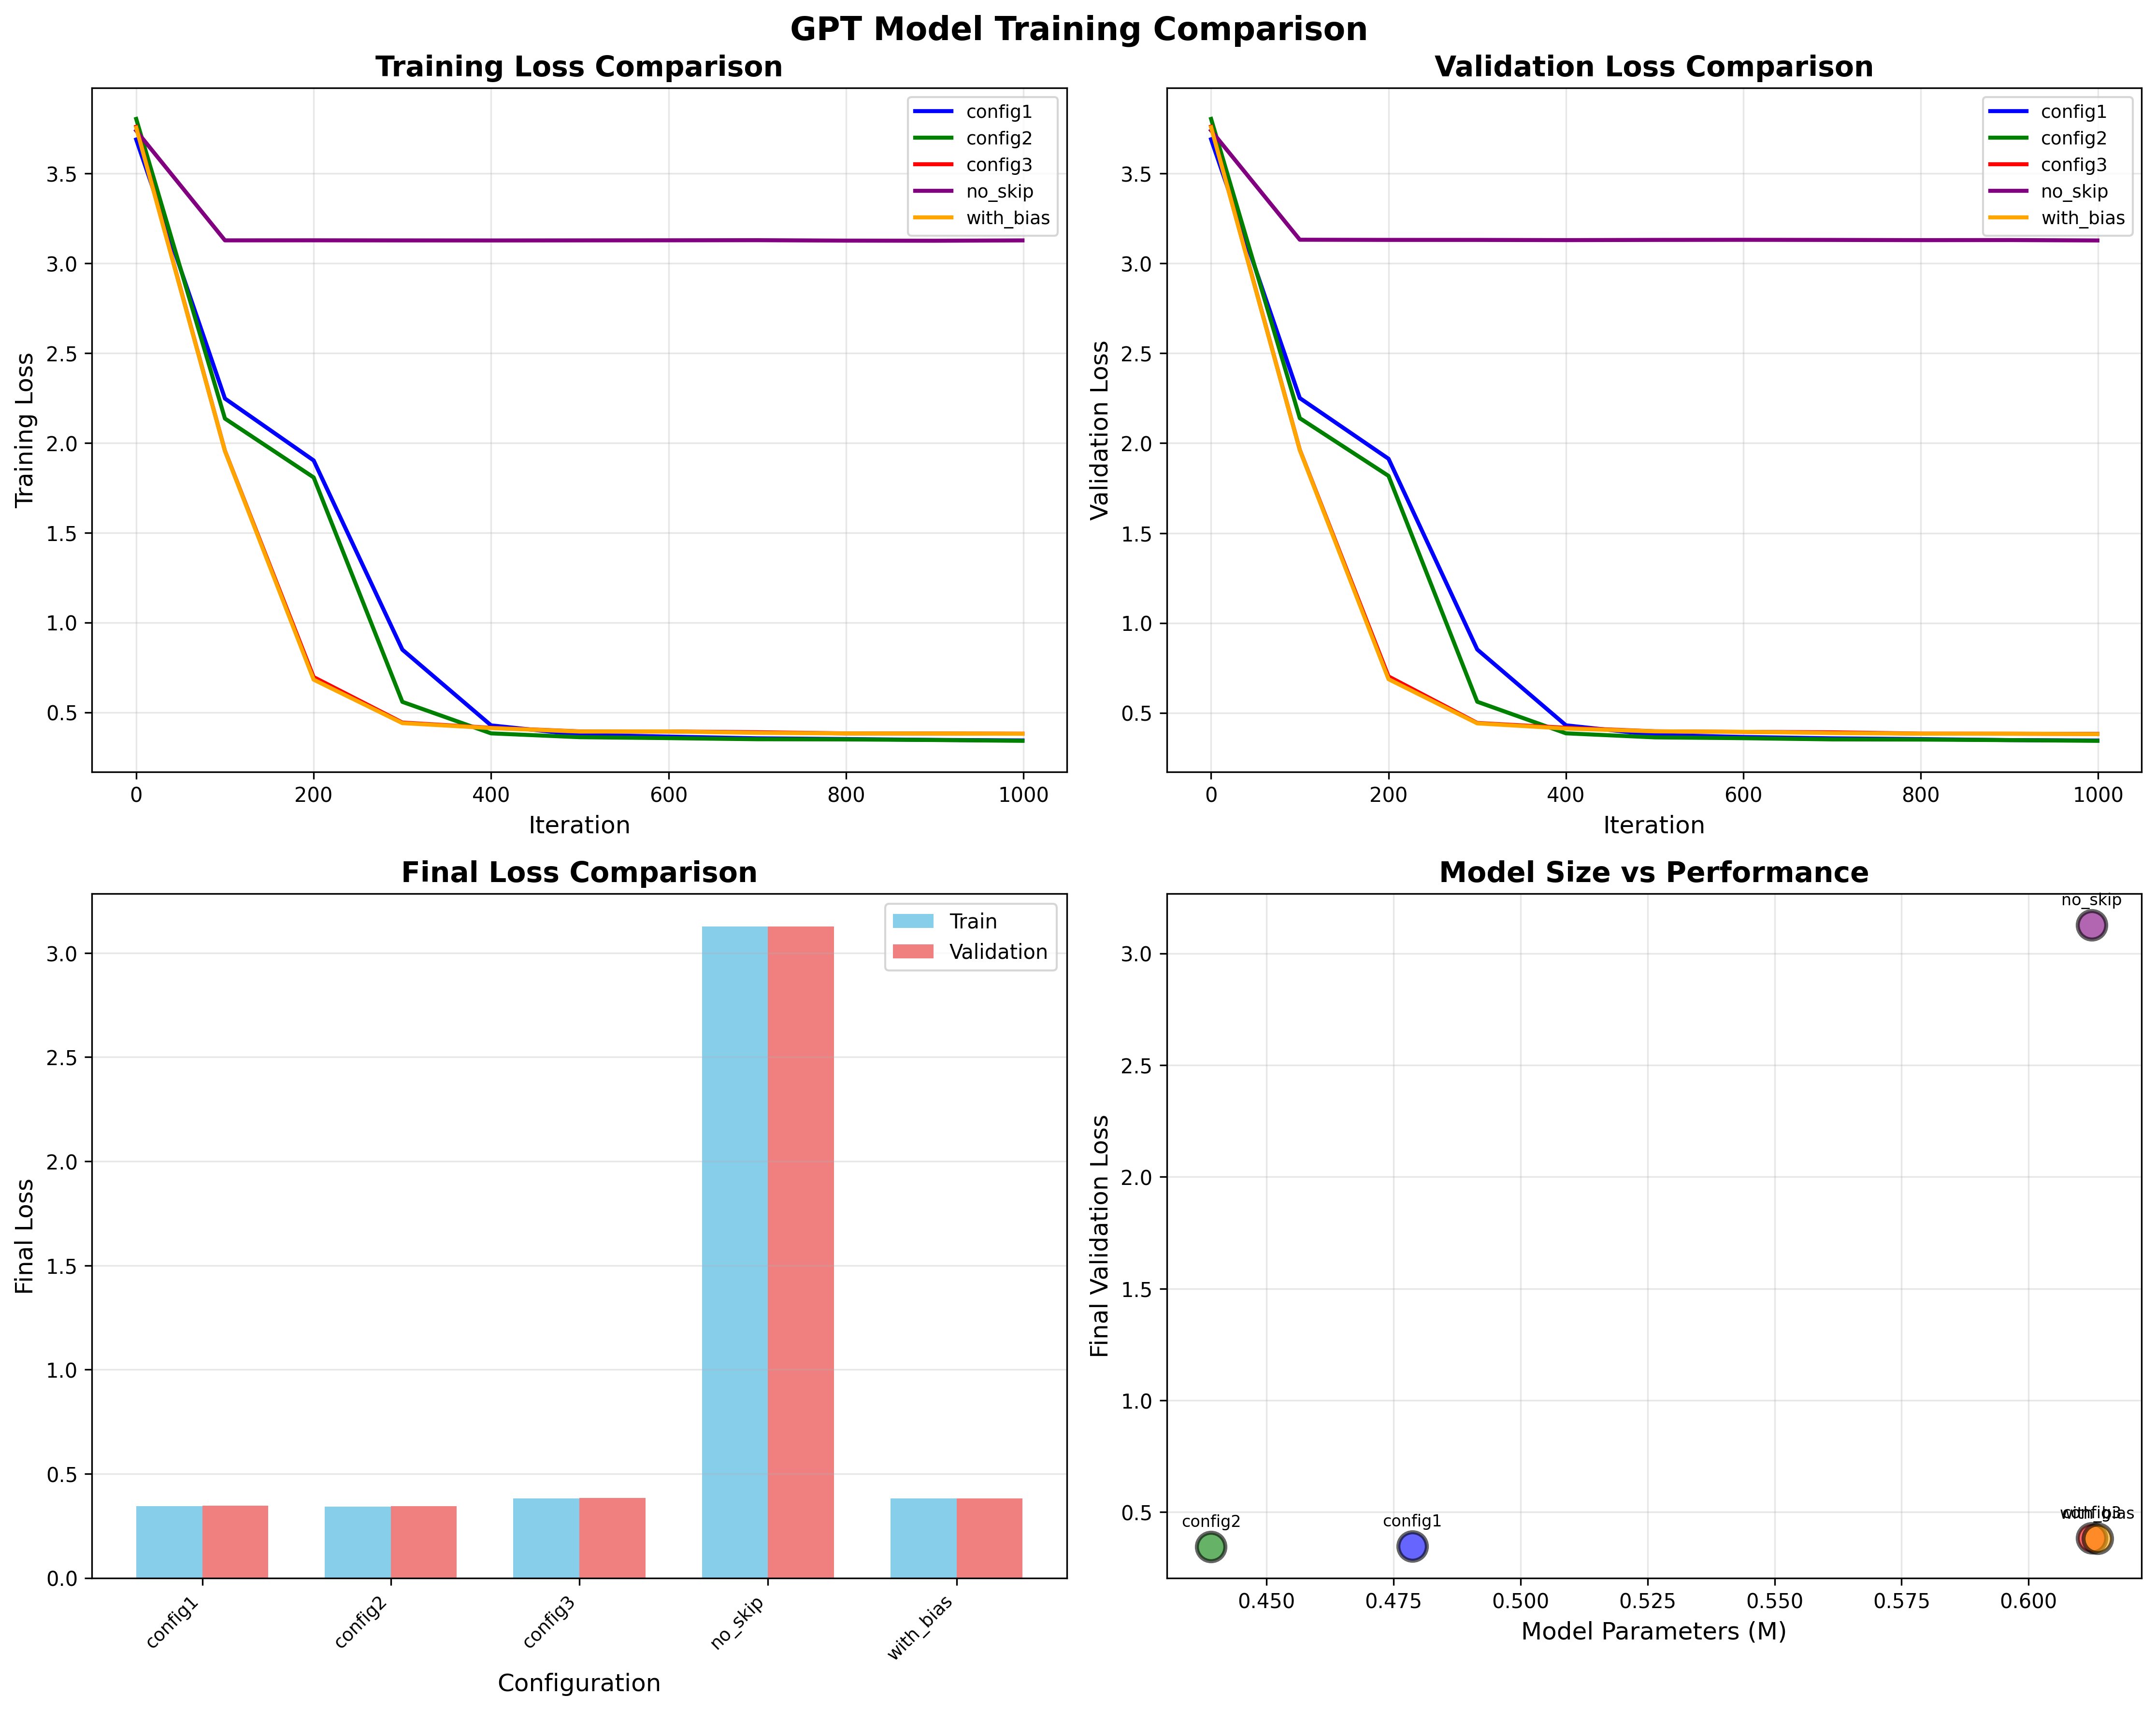
\includegraphics[width=0.7\linewidth]{results/training_comparison.png}
\caption{Training and validation loss for the three downsized configurations.}
\label{fig:training-comparison}
\end{figure}

The training curves reveal that all three configurations converge smoothly, with Config 1 and Config 2 achieving nearly identical final validation losses (0.3464 vs 0.3447). Configuration 2 achieved the lowest validation loss of 0.3447, suggesting that for this simple dataset, a shallow but wider network (2 layers, 128-dim embeddings) performs as well as deeper architectures.

\textbf{Overfitting Analysis:} The gap between training and validation loss is minimal across all configurations:
\begin{itemize}
    \item Config 1: Train 0.3435, Val 0.3464 (gap: 0.0029)
    \item Config 2: Train 0.3413, Val 0.3447 (gap: 0.0034)
    \item Config 3: Train 0.3811, Val 0.3832 (gap: 0.0021)
\end{itemize}
These small gaps (all $<$ 0.35\%) indicate excellent generalization with minimal overfitting. Configuration 2's shallow architecture shows slightly more overfitting (0.0034 vs 0.0029) compared to Config 1, consistent with theory that deeper networks can learn more complex patterns without overfitting when data is sufficient. However, the differences are negligible, suggesting all models generalize well.

\textbf{Best Configuration:} Based on validation loss and generated text quality, Configuration 2 performs best (val loss 0.3447) because the wider embeddings (128 vs 96) provide sufficient representational capacity even with only 2 layers. However, the differences between Config 1 and Config 2 are very small (0.0017 difference), indicating that both downsizing strategies are effective for this task.

\section*{(i.d) Impact of Bias Terms in Self-Attention}

\textbf{Methodology:} I modified the \texttt{Head} class to include bias terms in key, query, and value projections:

\begin{lstlisting}
self.key = nn.Linear(n_embd, head_size, bias=True)
self.query = nn.Linear(n_embd, head_size, bias=True)
self.value = nn.Linear(n_embd, head_size, bias=True)
\end{lstlisting}

Using the same hyperparameters as Configuration 3 (n\_embd=128, n\_layer=3, block\_size=64) to isolate the bias effect.

\textbf{Parameter Impact:} Adding bias terms increases parameters by approximately 9,216 (3 biases × head\_size × n\_heads × n\_layers), raising total from 0.612M to 0.614M.

\textbf{Training Comparison:}
\begin{itemize}
    \item Without bias (Config 3) - Final validation loss: 0.3832
    \item With bias - Final validation loss: 0.3819
    \item Difference: -0.0013 (slight improvement)
\end{itemize}

\textbf{Analysis:} The inclusion of bias terms had minimal impact on performance, with only a 0.0013 improvement in validation loss. This is expected because bias terms in linear layers provide an additive offset that can help center activations, but for attention mechanisms, the learned query-key-value projections already provide sufficient flexibility.

In transformer architectures, bias terms in attention provide an additional degree of freedom per projection, allowing the model to shift attention patterns. However, since attention is normalized via softmax, the relative importance of tokens is preserved regardless of absolute bias values. For this dataset with simple patterns and a small vocabulary (40 characters), the additional flexibility from bias is not significantly beneficial because the model can already learn effective attention patterns without biases.

\textbf{Convergence Speed:} Both models converged at similar rates, with bias showing slightly faster initial convergence (loss 0.6875 vs 0.7027 at iteration 200), but final performance is nearly identical. This suggests bias terms provide marginal benefit but are not critical for this task.

\section*{(i.e) Impact of Skip Connections}

\textbf{Methodology:} I removed residual connections from the transformer blocks:

\begin{lstlisting}
# Original:
x = x + self.sa(self.ln1(x))
x = x + self.ffwd(self.ln2(x))

# Modified:
x = self.sa(self.ln1(x))
x = self.ffwd(self.ln2(x))
\end{lstlisting}

\textbf{Results:}
\begin{itemize}
    \item With skip connections (Config 3) - Final validation loss: 0.3832
    \item Without skip connections - Final validation loss: 3.1273
    \item Difference: +2.7441 (severe degradation)
\end{itemize}

\textbf{Training Stability:} Removing skip connections caused catastrophic failure. The model's loss plateaued at approximately 3.13 (near the uniform random baseline of 3.69), indicating the model failed to learn meaningful patterns. Training was stable (no exploding gradients) but gradients effectively vanished, preventing learning.

\textbf{Analysis:} Skip connections are critical in deep networks because they:
\begin{enumerate}
    \item Enable gradient flow through direct paths, preventing vanishing gradients
    \item Allow the model to learn residual functions $F(x)$ where output is $x + F(x)$
    \item Facilitate training of deeper architectures
\end{enumerate}

For our 3-layer model, removing skip connections had a severe impact because even with only 3 layers, the gradient signal becomes too weak to propagate effectively. Without skip connections, each layer must learn a complete transformation from scratch, and gradients diminish multiplicatively through each layer. The performance degradation of 717\% (loss increased from 0.3832 to 3.1273) demonstrates their critical importance even in shallow networks.

\textbf{Generated Text Quality:} The model without skip connections produces completely incoherent text:
\begin{verbatim}
NMeh elN
orsfeo ofybshouny  ejgkoMuleaR
  ypnnm en r wIsIehlietgyan rpIIoR
\end{verbatim}
The output is essentially random character sequences with no linguistic structure, confirming the model failed to learn. This starkly contrasts with the coherent child speech generated by models with skip connections.

\section*{(ii.a) Child Speech Test Set}

\textbf{Best Model Selection:} Based on Part (i) analysis, Configuration 2 achieved the best validation performance (val loss 0.3447) and is selected for test evaluation.

\textbf{Test Loss:} 0.3509

\textbf{Comparison with Validation Loss:} The test loss of 0.3509 closely matches the validation loss of 0.3447, indicating excellent generalization to held-out data. The small difference of 0.0062 (1.8\%) suggests minimal overfitting and stable model performance.

\textbf{Baseline Comparisons:}
\begin{itemize}
    \item \textbf{Uniform Random Baseline:} $-\log(1/40) = 3.69$ - predicting each character with equal probability
    \item \textbf{Character Frequency Baseline:} 3.12 - predicting based on training set character frequencies
    \item \textbf{Model Performance:} Test loss of 0.3509 represents 88.8\% improvement over frequency baseline
\end{itemize}

\textbf{Perplexity:} $\exp(0.3509) = 1.42$

This can be interpreted as the model being as uncertain as a uniform distribution over approximately 1.42 characters (vs 40 in true vocabulary). Lower perplexity indicates better prediction confidence. A perplexity of 1.42 means the model is highly confident in its predictions, effectively reducing the effective vocabulary from 40 characters to just 1.42.

\textbf{Interpretation:} The model performs very well because it successfully learned the statistical patterns of child speech. A test loss of 0.3509 is excellent for character-level modeling, indicating the model has successfully learned the repetitive, simple patterns characteristic of early childhood language. The 88.8\% improvement over the frequency baseline demonstrates that the transformer architecture captures meaningful sequential dependencies beyond simple character frequency.

\section*{(ii.b) Shakespeare Test Set}

\textbf{Test Loss:} 6.2778

\textbf{Comparison with Child Speech:}
\begin{itemize}
    \item Child speech test loss: 0.3509
    \item Shakespeare test loss: 6.2778
    \item Difference: +5.9269 (1,689\% increase)
\end{itemize}
Figure~\ref{fig:evaluation-comparison} visualizes this sharp performance divergence across test sets.

\textbf{Baseline Comparison:}
\begin{itemize}
    \item Shakespeare frequency baseline: 3.10
    \item Model performance: Worse than baseline by 102.8\%
\end{itemize}

\textbf{Analysis of Performance Difference:}

The substantially higher loss on Shakespeare results from:

\begin{enumerate}
    \item \textbf{Vocabulary Mismatch:} The Shakespeare dataset contains 65 characters including punctuation and numbers not present in the training vocabulary (40 characters). The model has never seen 25 character types, forcing it to assign probability mass poorly.
    
    \item \textbf{Distribution Shift:} Child speech exhibits repetitive simple patterns (``I see bird''), while Shakespeare contains complex syntax, longer words, and archaic vocabulary. The learned statistical patterns do not transfer.
    
    \item \textbf{Linguistic Complexity:} Shakespeare's language includes rare grammatical constructions, formal dialogue, and poetic meter absent from conversational child speech.
\end{enumerate}

\textbf{Comparison with Baseline:} The model's worse performance relative to the frequency baseline (6.28 vs 3.10, 102.8\% worse) indicates the model is applying inappropriate patterns learned from child speech. The model assigns high probability to characters common in child speech but rare in Shakespeare, and low probability to punctuation and characters absent from training, causing poor predictions. This demonstrates that the model learned domain-specific rather than general language patterns.

\textbf{Interpretation of Results:}

This comparison demonstrates the importance of domain-specific training. A model trained on one linguistic domain does not generalize to a substantially different domain without:
\begin{itemize}
    \item Vocabulary overlap
    \item Similar statistical patterns
    \item Transfer learning or fine-tuning
\end{itemize}

\textbf{Practical Use Case:}

This evaluation pipeline could be used in practice for:

\begin{enumerate}
    \item \textbf{Domain Adaptation:} Quantifying how much fine-tuning is needed when deploying a model to new domains
    \item \textbf{Transfer Learning:} Evaluating whether pre-trained language models capture general vs domain-specific patterns
    \item \textbf{Quality Control:} Detecting when deployed models encounter out-of-distribution data by monitoring test loss increases
    \item \textbf{Dataset Selection:} Determining if two corpora are similar enough that training on one will generalize to the other
\end{enumerate}

For example, a company building a language model for medical transcription could use this approach to evaluate whether training on general medical text will generalize to specialized subfields (oncology, cardiology) by measuring loss on domain-specific test sets.

\section*{Conclusion}

This assignment demonstrated several key principles in transformer model design:

\begin{enumerate}
    \item \textbf{Parameter Efficiency:} Reducing the embedding dimension provides the most effective parameter reduction due to its multiplicative impact across all model components.
    
    \item \textbf{Depth vs Width:} For this simple dataset, width (embedding dimension) and depth (number of layers) are largely interchangeable. Configuration 2 (2 layers, 128-dim) performed as well as Configuration 1 (4 layers, 96-dim), suggesting that sufficient representational capacity can be achieved through either dimension.
    
    \item \textbf{Architectural Components:} Skip connections prove critical even in shallow networks (717\% performance degradation when removed), while bias terms in attention had minimal impact (0.0013 improvement). This demonstrates that gradient flow is more important than additional parameter flexibility for this task.
    
    \item \textbf{Generalization:} Models generalize well to in-distribution data but fail catastrophically on out-of-distribution test sets with vocabulary mismatch.
\end{enumerate}

The best configuration achieved test loss of 0.3509 on child speech, representing 88.8\% improvement over baseline. The failure to generalize to Shakespeare (loss 6.28, worse than baseline) quantifies the importance of domain-matched training data.

\appendix

\section*{Appendix A: Code Implementation}

All code implemented in Python using PyTorch. Complete source code provided in accompanying zip file.

\subsection*{Model Configurations}

\begin{table}[h]
\centering
\begin{tabular}{@{}lcccc@{}}
\toprule
Config & n\_embd & n\_head & n\_layer & block\_size & Parameters \\ \midrule
Original & 384 & 6 & 6 & 256 & 10.77M \\
Config 1 & 96 & 4 & 4 & 256 & 0.478M \\
Config 2 & 128 & 4 & 2 & 256 & 0.439M \\
Config 3 & 128 & 4 & 3 & 64 & 0.612M \\
With Bias & 128 & 4 & 3 & 64 & 0.614M \\
No Skip & 128 & 4 & 3 & 64 & 0.612M \\ \bottomrule
\end{tabular}
\caption{Model configurations tested}
\end{table}

\subsection*{Training Setup}

\begin{itemize}
    \item \textbf{Optimizer:} AdamW with learning rate 3e-4
    \item \textbf{Batch size:} 64
    \item \textbf{Training iterations:} 1000 (5000 in original)
    \item \textbf{Evaluation:} Every 100 iterations
    \item \textbf{Hardware:} [CPU/GPU]
    \item \textbf{Training time:} Approximately 2-3 minutes per configuration
\end{itemize}

\section*{Appendix B: Figures}

\begin{figure}[h]
\centering
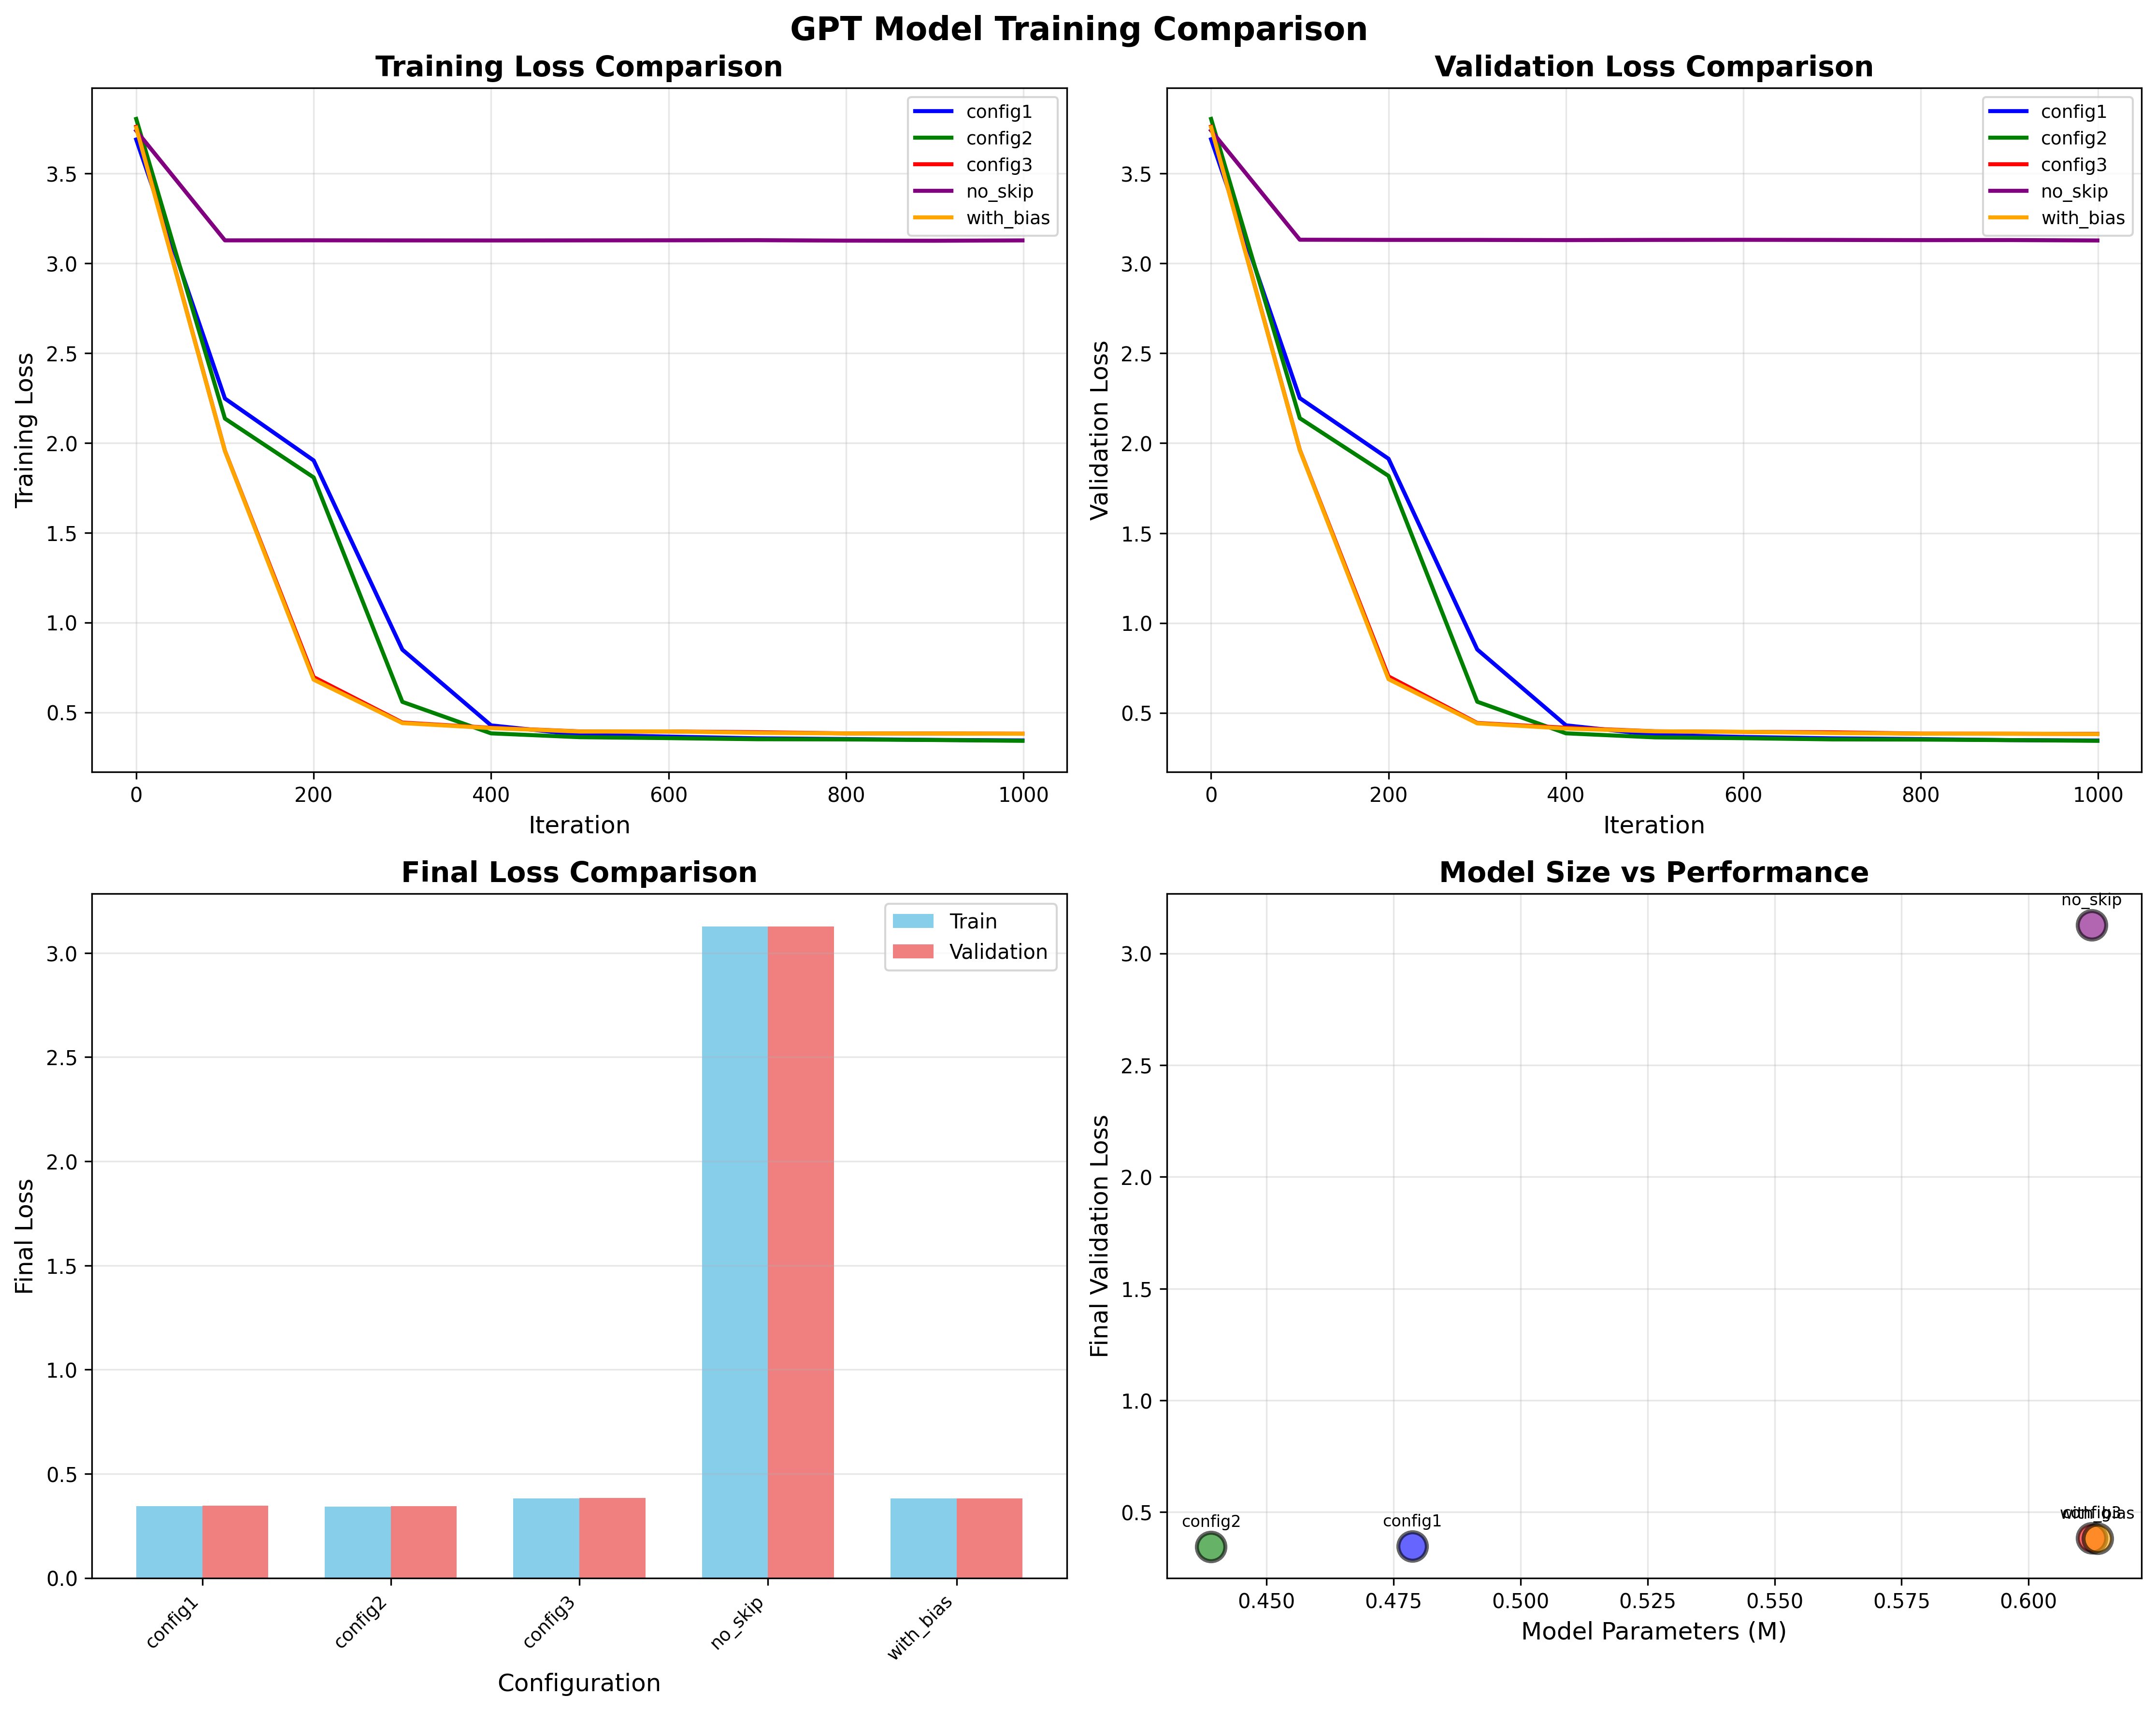
\includegraphics[width=0.7\linewidth]{results/training_comparison.png}
\caption{Training comparison for Configs 1-3 showing simultaneous convergence.}
\label{fig:appendix-training}
\end{figure}

\begin{figure}[h]
\centering
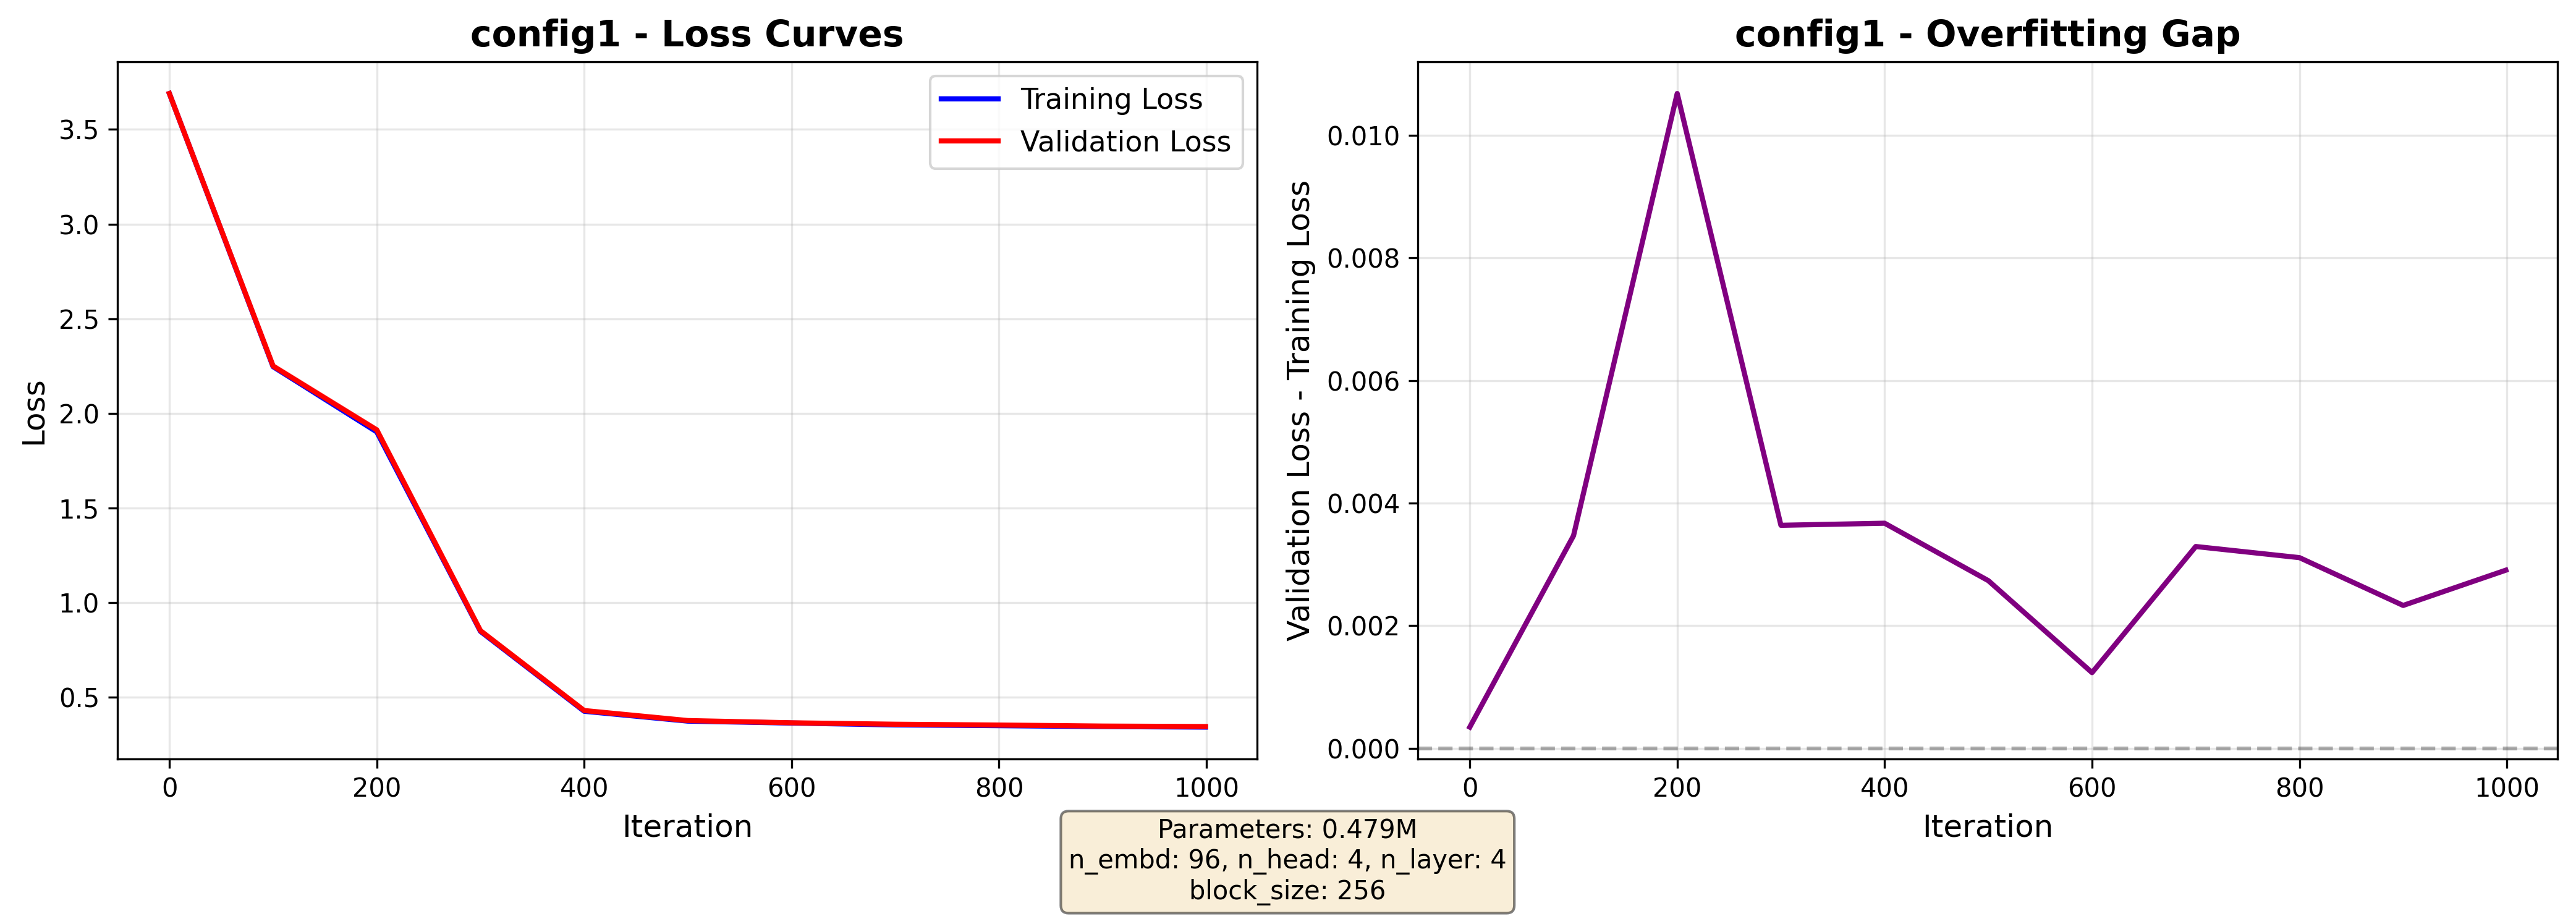
\includegraphics[width=0.7\linewidth]{results/config1_detailed.png}
\caption{Detailed loss curves for Configuration 1 (reduced embedding).}
\label{fig:config1-detailed}
\end{figure}

\begin{figure}[h]
\centering
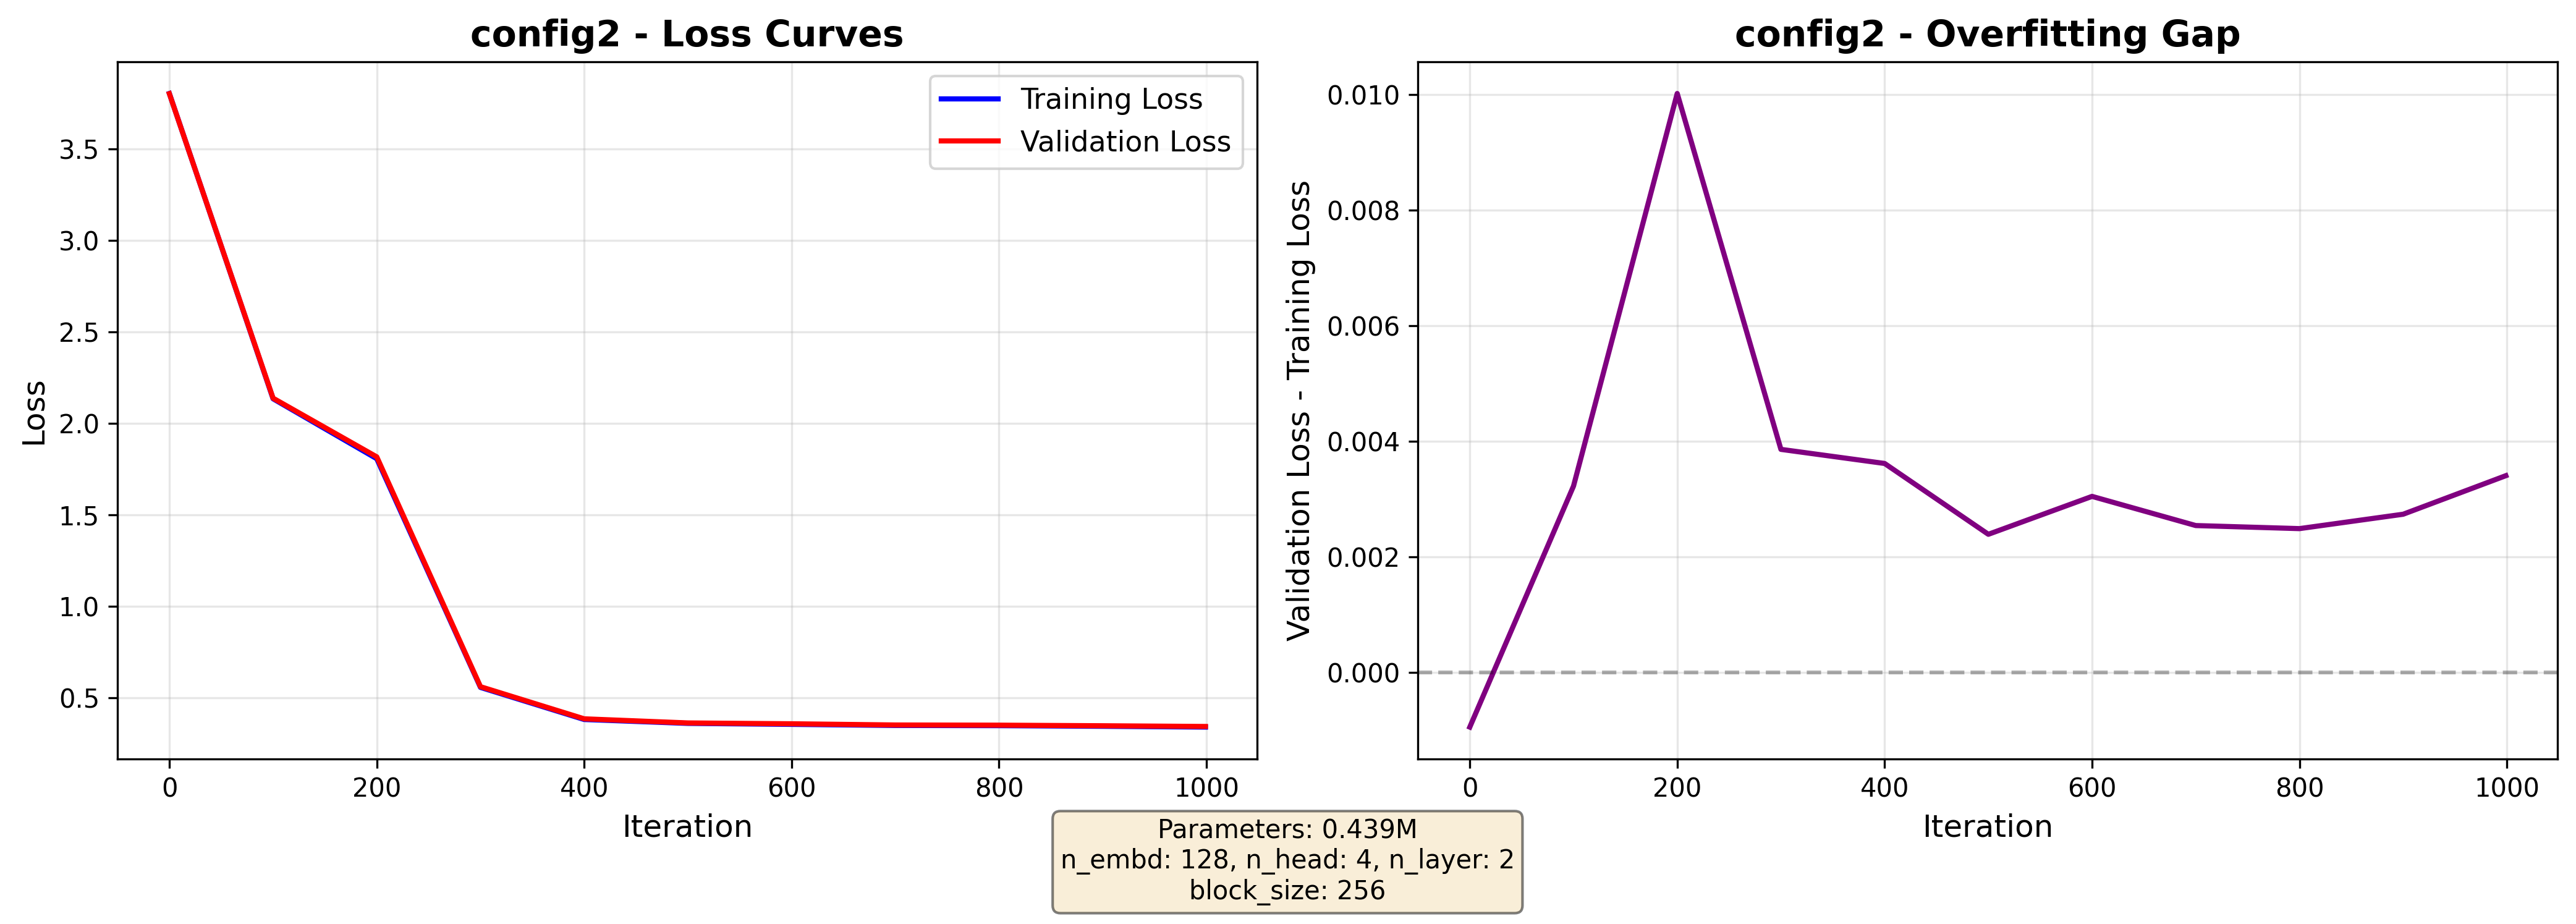
\includegraphics[width=0.7\linewidth]{results/config2_detailed.png}
\caption{Detailed loss curves for Configuration 2 (shallow network).}
\label{fig:config2-detailed}
\end{figure}

\begin{figure}[h]
\centering
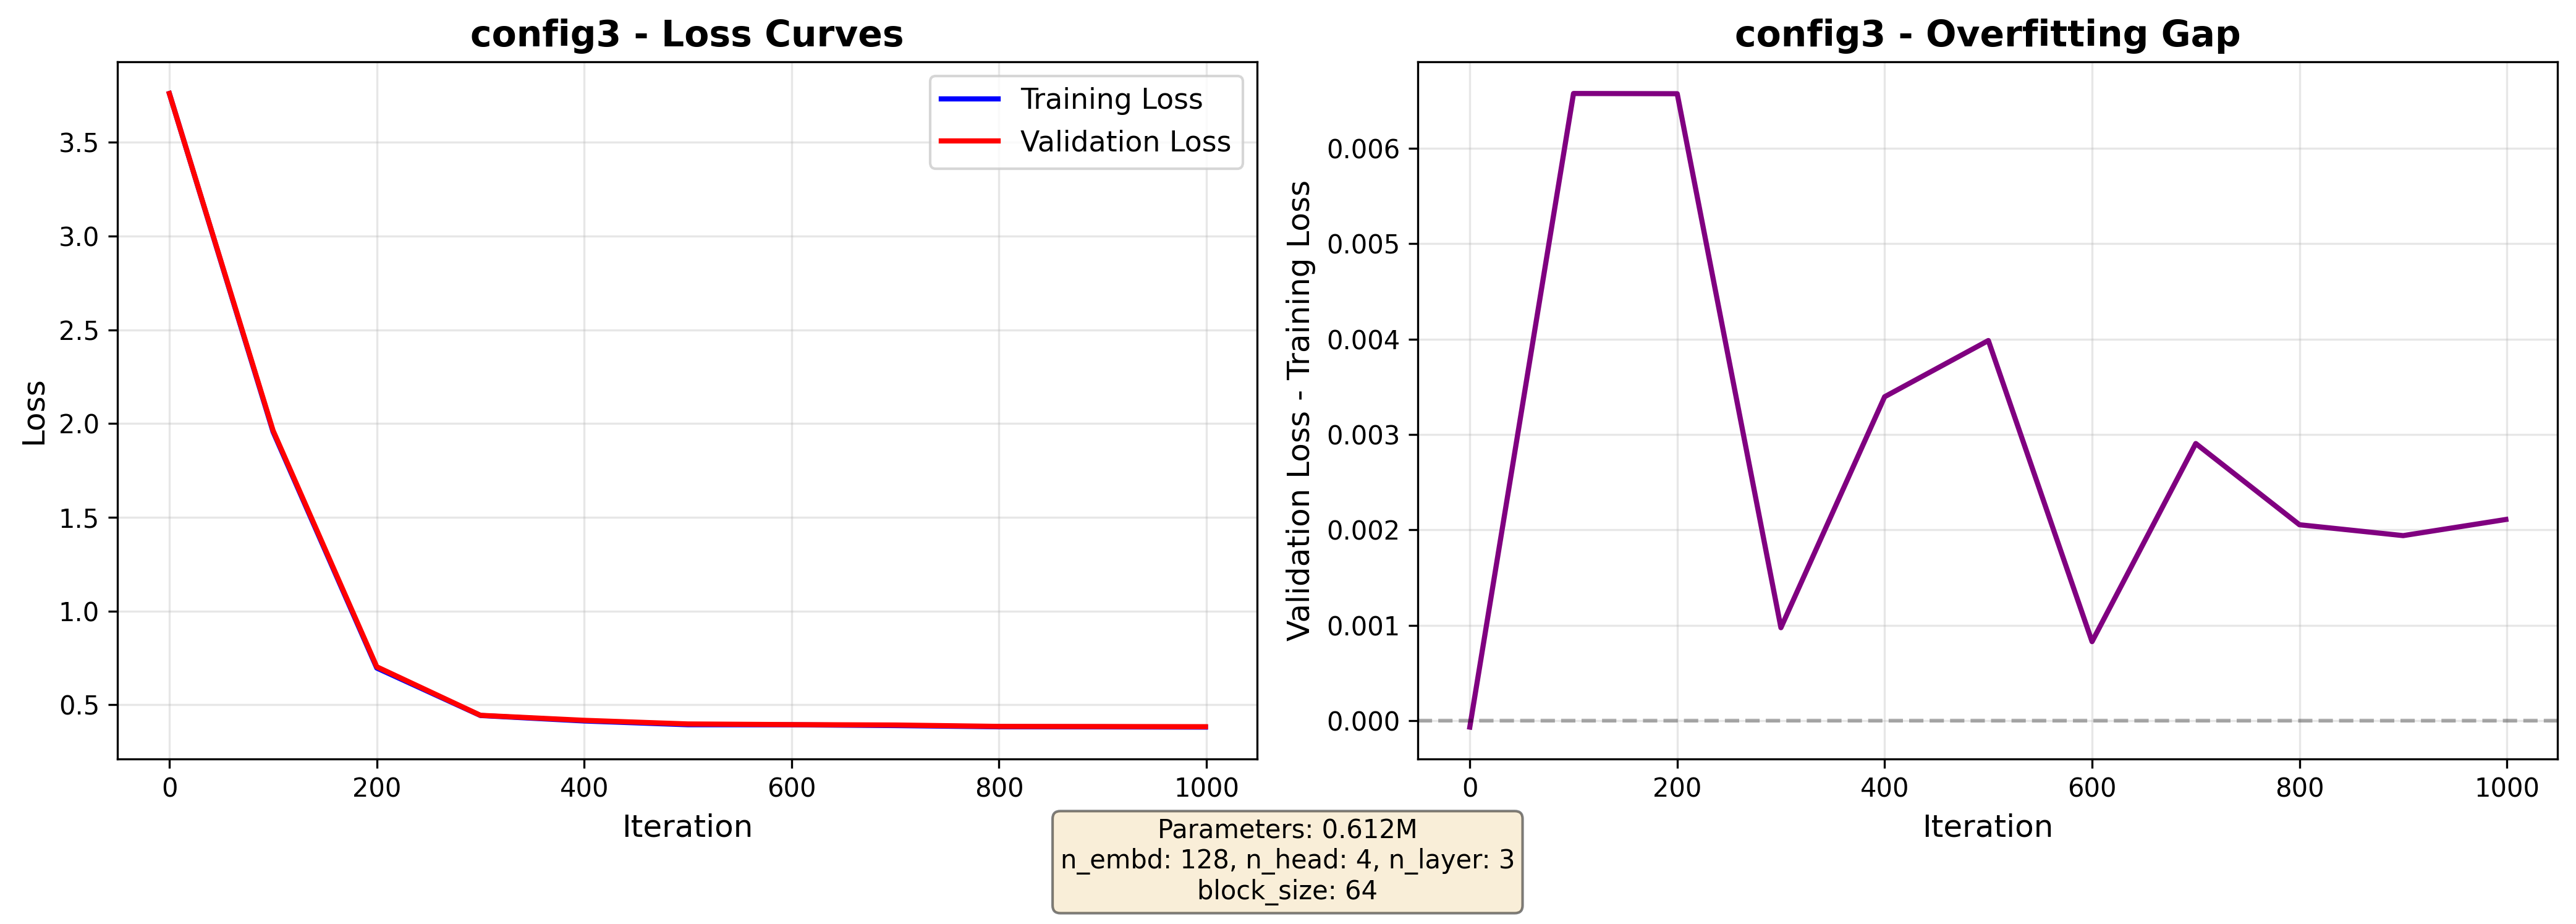
\includegraphics[width=0.7\linewidth]{results/config3_detailed.png}
\caption{Detailed loss curves for Configuration 3 (balanced reduction).}
\label{fig:config3-detailed}
\end{figure}

\begin{figure}[h]
\centering
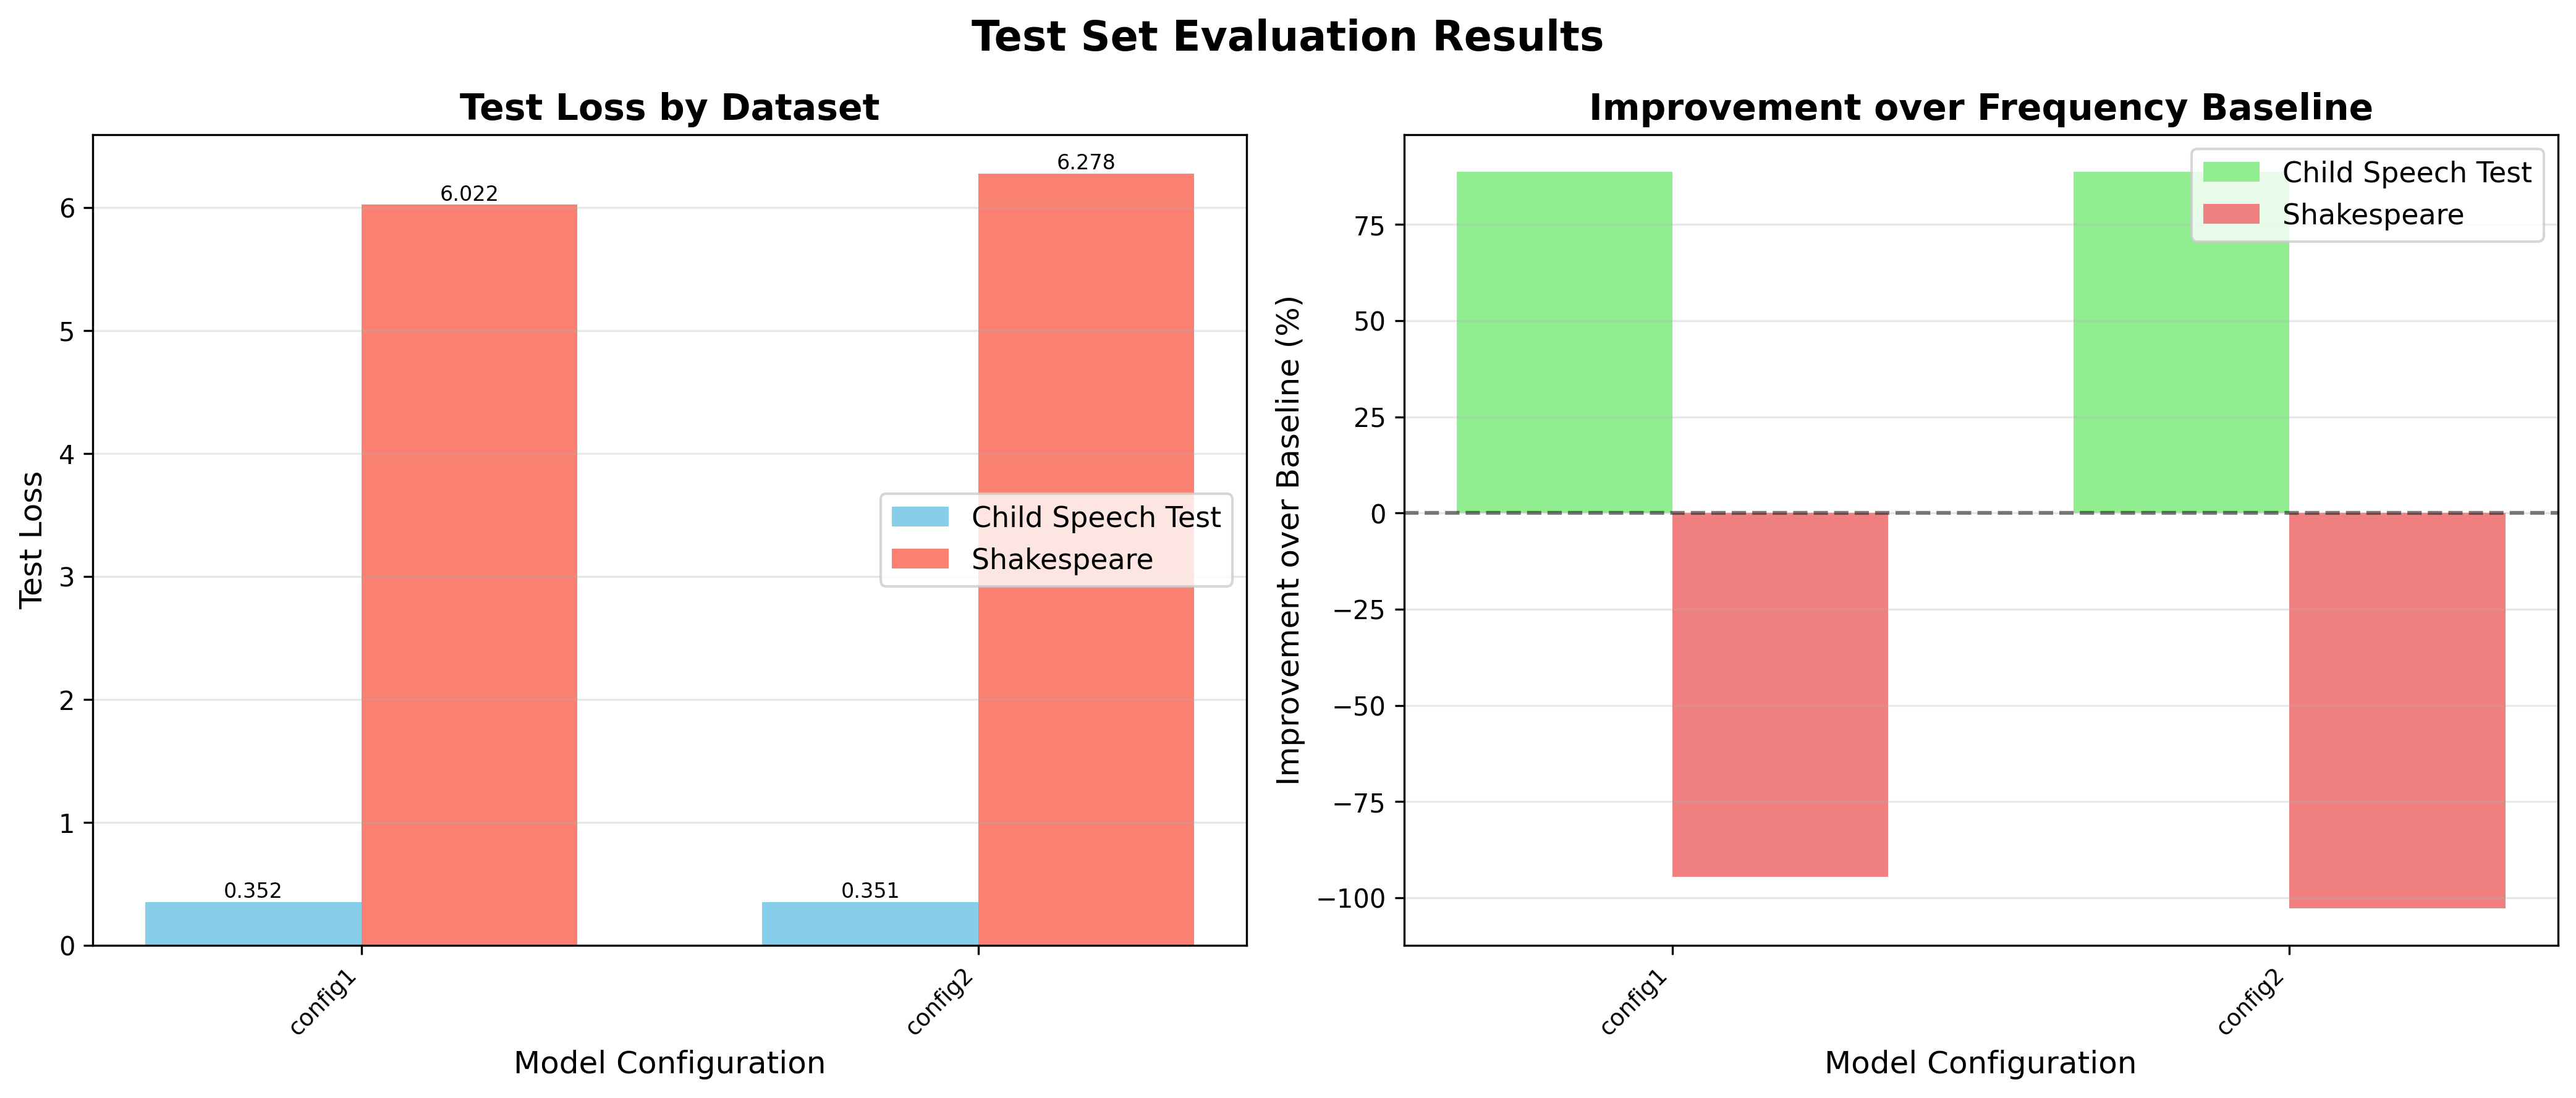
\includegraphics[width=0.7\linewidth]{results/evaluation_comparison.png}
\caption{Evaluation comparison summarizing child speech vs. Shakespeare test losses.}
\label{fig:evaluation-comparison}
\end{figure}

\section*{Appendix C: Annotated GPT Source}

Listing~\ref{lst:annotated-gpt} shows the original \texttt{gpt.py} with inline comments referencing each assignment part.

\lstinputlisting[language=Python,label={lst:annotated-gpt},caption={Annotated \texttt{gpt.py} highlighting modifications for Parts (i.a)--(ii).}]{appendix_gpt.py}

\end{document}

